\documentclass[a4paper]{article}

\usepackage[text={18.6cm, 26.0cm}, centering]{geometry}

\usepackage[czech, provide=*]{babel}
\usepackage[utf8]{inputenc}
\usepackage[T1]{fontenc}
\usepackage{color}
\usepackage{alltt} % \verb
\usepackage[hidelinks]{hyperref} % odkazy
\usepackage{tikz}

% Ceske uvozovky
\providecommand{\uv}[1]{\quotedblbase #1\textquotedblleft}

\begin{document}
    \begin{titlepage}
        \begin{center}
            \textsc{\Huge{}Vysoké učení technické v Brně\\[0.5em]}
            \textsc{\huge Fakulta informačních technologií}\\
            \vspace{\stretch{0.382}}
            { \huge Wren překladač\,--\,dokumentace\\[0.5em]
                IFJ/IAL 2025 }\\[0.5em]
                Tým xsebesm00, varianta TRP-izp\\
            \vspace{\stretch{0.618}}
        \end{center}
        { \phantom{a}\hfill FUNEXP\\
          \phantom{a}\hfill EXTSTAT\\
          Vojtěch Borýsek (xborysv00)\,--\, 33\% \hfill EXTFUN\\
          Šimon Halas (xhalass00)\,--\, 00\% \hfill BOOLTHEN\\
          Tomáš Hanák (xhanakt00)\,--\, 33\% \hfill OPERATORS\\
          Michal Šebesta (xsebesm00)\,--\, 34\%, vedoucí \hfill STATICAN\\
          }
    \end{titlepage}
    \tableofcontents
    \newpage
    \section{Přehled}
        \begin{center}
            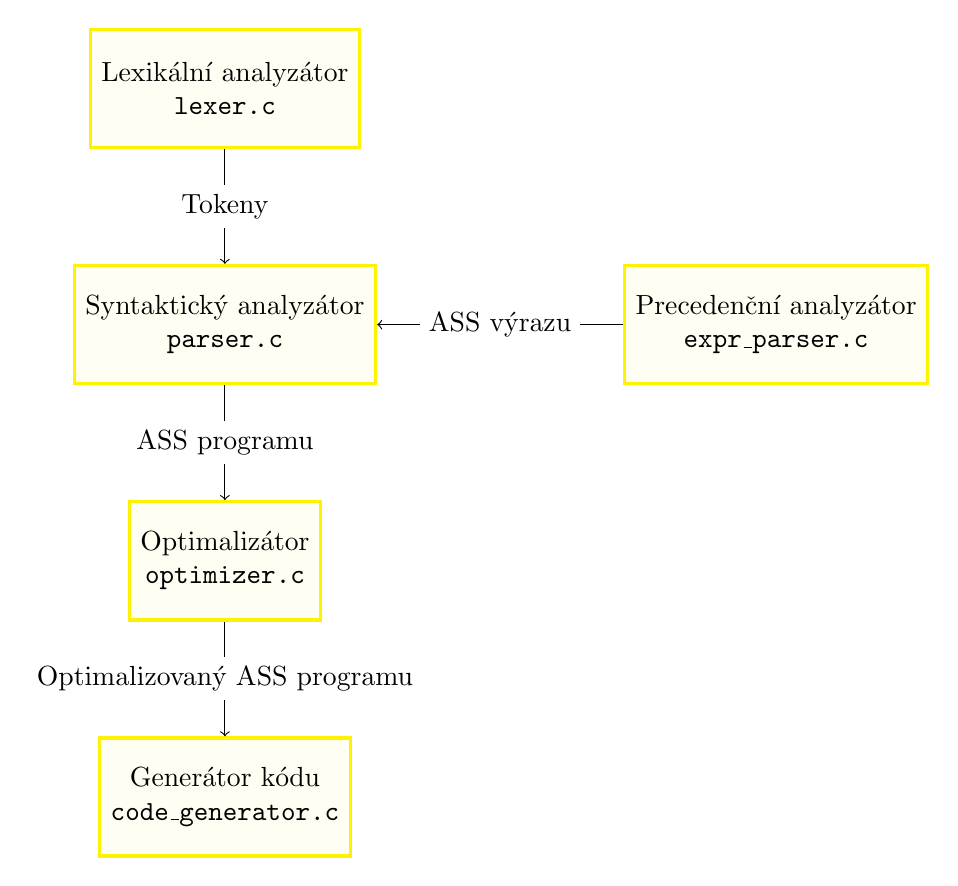
\begin{tikzpicture}[
                    every node/.style={fill=white},
                    block/.style={rectangle, draw=yellow, fill=yellow!5, very thick, minimum size=15mm, inner sep=4pt,draw},
                    node distance=3cm,
                    align=center,
                ]
                \node[block] (lexer) {Lexikální analyzátor\\ \texttt{lexer.c}};
                \node[block] (parser) [below of=lexer] {Syntaktický analyzátor\\ \texttt{parser.c}};
                \node[block] (expr) [right of=parser, xshift=4cm]{Precedenční analyzátor\\ \texttt{expr\_parser.c}};
                \node[block] (optimizer) [below of=parser] {Optimalizátor\\ \texttt{optimizer.c}};
                \node[block] (codegen) [below of=optimizer] {Generátor kódu\\ \texttt{code\_generator.c}};

                \draw[->] (lexer.south) -- node {Tokeny} (parser.north);
                \draw[->] (expr.west) -- node {ASS výrazu} (parser.east);
                \draw[->] (parser.south) -- node {ASS programu} (optimizer.north);
                \draw[->] (optimizer.south) -- node {Optimalizovaný ASS programu} (codegen.north);
            \end{tikzpicture}
        \end{center}
        Překlad začíná inicializací lexikálního analyzátoru. Ten je následně předán syntaktickému analyzátoru,
        který jej volá v případě potřeby tokenu. Pokud syntaktický analyzátor potřebuje načíst výraz, volá precedenční
        analyzátor. V rámci syntaktického analyzátoru se rovnou také provádí sémantické akce,
        jako kontrola typů výrazů, nebo kontrola deklarace proměnných. Výsledek ukládá do abstraktního
        syntaktického stromu (ASS).

        Jakmile je celý program převeden na ASS a sémanticky zkontrolován, je tento strom předán do optimalizátoru, který strom zoptimalizuje.
        Optimalizovaný strom je následně předán generátoru kódu, který z něj vytvoří cílový kód, čímž překlad končí.


    \section{Lexikální analýza}
        TODO

    \section{Syntaktický analýza}
        TODO
    \subsection{Tabulka symbolů}
        TODO
    \subsection{Sémantická analýza}
        TODO
    \subsection{Zpracování výrazů}
        TODO
    \subsection{Abstraktní syntaktický strom}
        TODO

    \section{Optimalizátor}
        Optimalizátor provádí optimalizaci abstraktního syntaktického stromu před jeho předáním generátoru kódu.
        Hlavním cílem je zjednodušení výrazů, které lze vyhodnotit již v době překladu, a tím snížení složitosti
        výsledného kódu a zvýšení rychlosti běhu programu.

        \subsection{Princip činnosti}
        Optimalizátor prochází celý AST rekurzivně a pro každý uzel provádí následující operace:
        \begin{enumerate}
            \item Nejprve optimalizuje všechny potomky uzlu (výrazy, příkazy, bloky)
            \item Pokud jsou všechny operandy výrazu známé v době překladu, pokusí se výraz vyhodnotit
            \item Udržuje informace o hodnotách proměnných v tabulce symbolů pro využití při optimalizaci
            \item Při operacích s vedlejšími efekty (volání funkcí, setterů) maže známé hodnoty proměnných
        \end{enumerate}

        \subsection{Typy optimalizací}
        \subsubsection{Konstantní výrazy}
        Optimalizátor vyhodnocuje výrazy, jejichž všechny operandy jsou konstanty:
        \begin{itemize}
            \item \textbf{Aritmetické operace}: \texttt{2 + 3} $\rightarrow$ \texttt{5}, \texttt{10 / 2} $\rightarrow$ \texttt{5.0}
            \item \textbf{Logické operace}: \texttt{true \&\& false} $\rightarrow$ \texttt{false}, \texttt{!true} $\rightarrow$ \texttt{false}
            \item \textbf{Porovnávání}: \texttt{5 > 3} $\rightarrow$ \texttt{true}, \texttt{"abc" == "abc"} $\rightarrow$ \texttt{true}
            \item \textbf{Stringové operace}: \texttt{"hello" + " world"} $\rightarrow$ \texttt{"hello world"}, \texttt{"abc" * 3} $\rightarrow$ \texttt{"abcabcabc"}
            \item \textbf{Ternární operátor}: \texttt{true ? 1 : 2} $\rightarrow$ \texttt{1}
        \end{itemize}

        \subsubsection{Vestavěné funkce}
        Optimalizátor dokáže vyhodnotit volání vestavěných funkcí s konstantními parametry:
        \begin{itemize}
            \item \texttt{Ifj.floor(3.7)} $\rightarrow$ \texttt{3.0}
            \item \texttt{Ifj.length("hello")} $\rightarrow$ \texttt{5.0}
            \item \texttt{Ifj.substring("hello", 1, 4)} $\rightarrow$ \texttt{"ell"}
            \item \texttt{Ifj.strcmp("abc", "def")} $\rightarrow$ \texttt{-1.0}
            \item \texttt{Ifj.ord("A", 0)} $\rightarrow$ \texttt{65.0}
            \item \texttt{Ifj.chr(65)} $\rightarrow$ \texttt{"A"}
        \end{itemize}

        \subsubsection{Propagace konstant}
        Optimalizátor sleduje hodnoty proměnných a využívá je k další optimalizaci:
        \begin{alltt}
var x = 5
var y = x + 3  // y = 8 (známe hodnotu x)
var z = y * 2  // z = 16 (známe hodnotu y)
        \end{alltt}

        Pokud je hodnota proměnné známá, nahradí její použití přímo hodnotou, čímž umožní
        další optimalizace výrazů obsahujících tuto proměnnou.

        \subsection{Ošetření vedlejších efektů}
        Optimalizátor musí správně zacházet s operacemi, které mohou mít vedlejší efekty:
        \begin{itemize}
            \item \textbf{Volání funkcí a getterů}: Při volání funkce nebo getteru se maží všechny
            známé hodnoty globálních proměnných, protože funkce může tyto proměnné modifikovat.
            \item \textbf{Volání setterů}: Podobně jako u funkcí se maží hodnoty globálních proměnných.
            \item \textbf{Podmínky a cykly}: V podmínkách \texttt{if} se optimalizují obě větve, ale
            po optimalizaci se maží známé hodnoty proměnných, protože není jisté, která větev se vykoná.
            V cyklech \texttt{while} se hodnoty maží jak před, tak po optimalizaci těla cyklu.
        \end{itemize}

        \subsection{Implementace}
        Optimalizátor se skládá z několika klíčových funkcí:
        \begin{itemize}
            \item \texttt{optimize\_ast()}: Vstupní bod optimalizátoru, inicializuje optimalizaci celého programu
            \item \texttt{optimize\_statement()}: Optimalizuje jednotlivé příkazy (deklarace, přiřazení, podmínky, cykly)
            \item \texttt{optimize\_expression()}: Rekurzivně optimalizuje výrazy, vyhodnocuje známé operace
            \item \texttt{optimize\_block()}: Optimalizuje bloky příkazů
            \item \texttt{update\_symtable\_value()}: Ukládá známé hodnoty proměnných do tabulky symbolů
            \item \texttt{clear\_symtable\_values()}: Maže známé hodnoty při operacích s vedlejšími efekty
        \end{itemize}
    \section{Generátor kódu}
        TODO

    \section{Rozdělení práce}
        \textbf{Vojtěch Borýsek}: Implementace precedenční analýzy a datových struktur.\\
        \textbf{Šimon Halas}: Implementace tabulky symbolů. Hodnocení 0\% kvůli plánovanému ukončení studia.\\
        \textbf{Tomáš Hanák}: Implementace syntaktické a sémantické analýzy a optimalizátoru.\\
        \textbf{Michal Šebesta}: Implementace lexikálního analyzátoru a generátoru kódu.
\end{document}
